\documentclass[10pt]{article}
\usepackage[utf8]{inputenc}
\usepackage{listings}
\usepackage{float}
\usepackage{graphicx}
\usepackage{fullpage}
\usepackage{caption}
\usepackage{subcaption}
\usepackage{amsmath}
\usepackage{hyperref}
\usepackage{epstopdf}

%\renewcommand{\thesubsection}{\arabic{subsection}}
\renewcommand{\thesubsubsection}{\alph{subsubsection}}

\title{Signals and Systems Lab 1}
\author{Maikel Withagen (s1867733) \and Steven Bosch (s1861948)}
\date{\today}
\lstset{
frame=single,
numbers=left,
breaklines=true,
language=Matlab,
basicstyle=\footnotesize,
title=\lstname,
showstringspaces=false
}

\renewcommand{\thesubsection}{\small(\alph{subsection})}
\begin{document}
\maketitle

\section{Summing Sinusoids}
\subsection{}
Our implementation of the function gensinusoid is given in section A(a) of the appendix.

\subsection{}
Using the function given in the previous section we get the graph given in figure \ref{fig1b}. The amount of samples that corresponds to one oscillation is $f_s/f=8000/400=20$.
\begin{figure}[H]
  \centering
  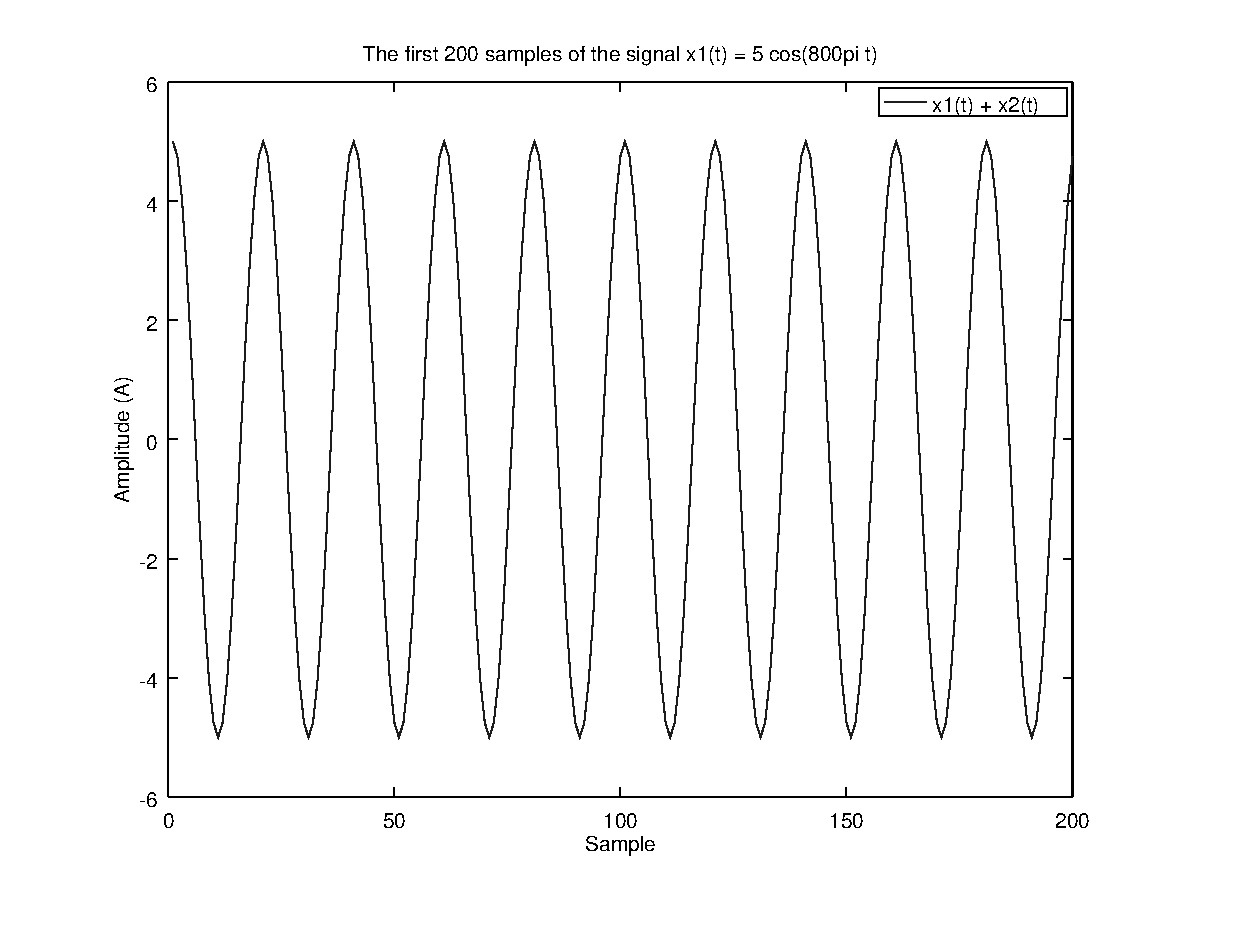
\includegraphics[width=.7\columnwidth]{plot1A.eps}
  \caption{The first 200 samples of the signal $x1(t) = 5cos(800\pi t)$}
  \label{fig1b}
\end{figure}

\subsection{}
Our implementation of the function sumsinusoid is given in section A(b) of the appendix.

\subsection{}
The shift of $0.013125s$ translates to a period of $\omega * t = 800\pi*0.013125 = 10.5\pi$. Now we have the following formulas:
\begin{equation}
    x1(t) = 5 cos(800\pi t)
\end{equation}
\begin{equation}
    x2(t) = 5 cos(800\pi t + 10.5\:pi)
\end{equation}
We can generate x1(t)+x2(t) by plotting the sum of the separate generated functions given by the function gensinusoid, resulting in figure \ref{fig2d1}.\\
\begin{figure}[H]
  \centering
  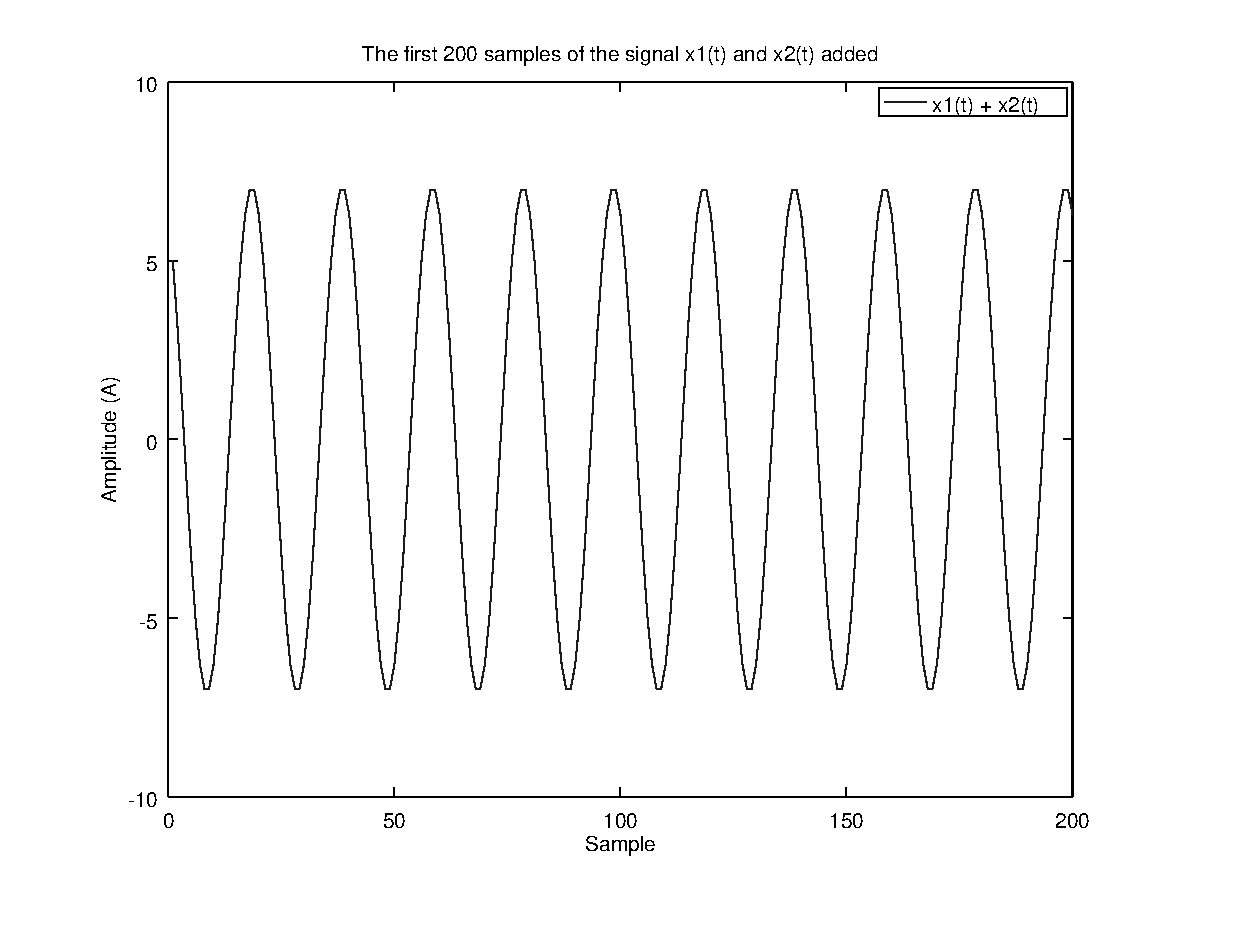
\includegraphics[width=.7\columnwidth]{plot4A.eps}\\
  \caption{The first 200 samples of the signal x1(t) and x2(t) added.}
  \label{fig2d1}
\end{figure}
Using the sumsinusoid function we can calculate the values for y(t):
$[A, f, phi] = 7.07107,400.00000,0.78540$, giving us\
\begin{equation}
    y(t) = 7.07107 cos(400*2*\pi t + 0.78540)
\end{equation}
The plot with both lines, given in figure \ref{fig2d2}, shows a perfect overlap, so we can conclude that our answer for y(t) is the same as the sum of the two functions. See section A(c) in the appendix for the script that executes the described process.

\begin{figure}[H]
  \centering
  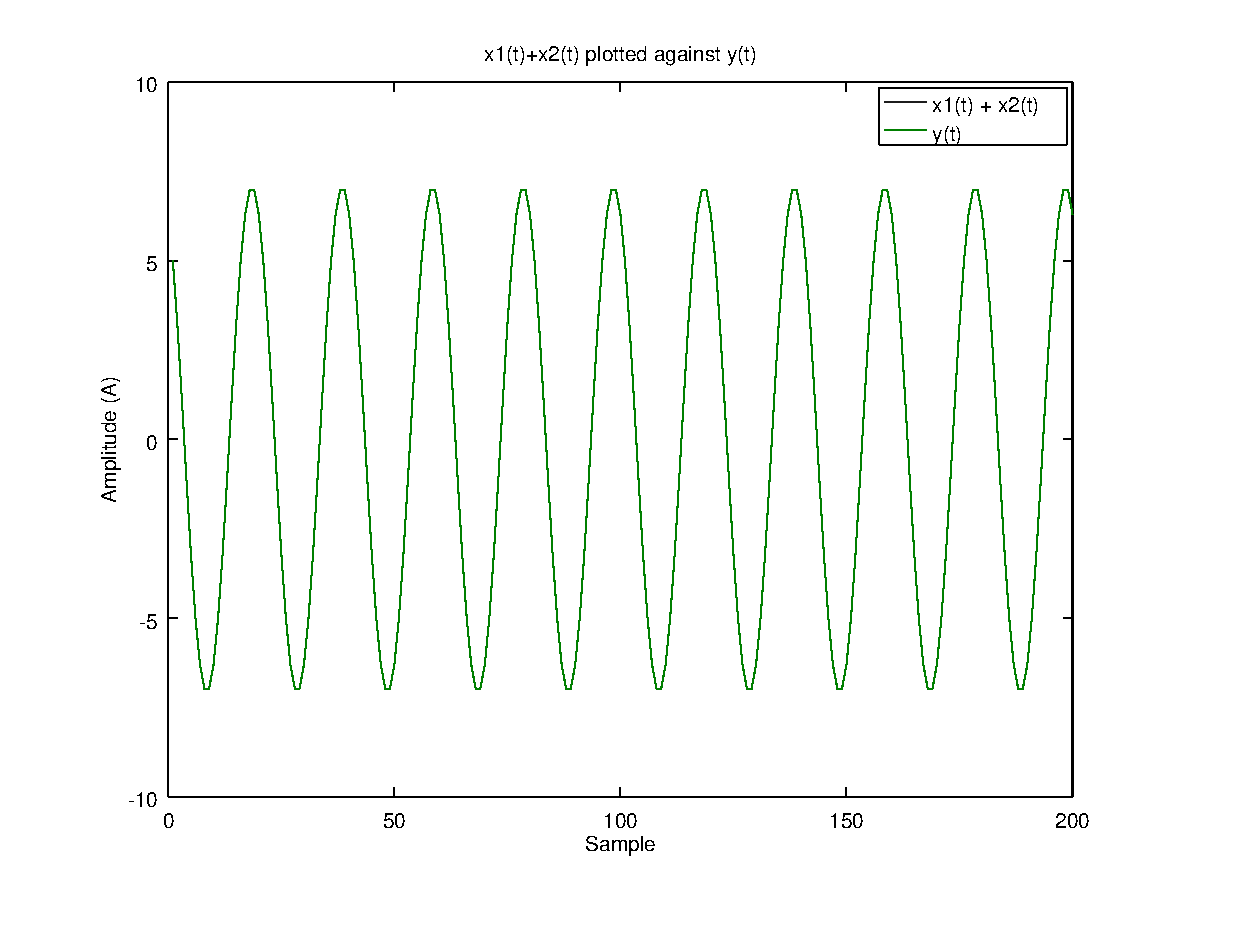
\includegraphics[width=.7\columnwidth]{plot4B.eps}
  \caption{x1(t)+x2(t) and y plotted in the same figure.}
  \label{fig2d2}
\end{figure}

\subsection{}
When we would combine signals $x1(t) = 5cos(800 \pi t)$ and $x3(t) = cos (1600 \pi t)$ we expect the following would happen: Since the frequency of $x3$ is twice as high as that of $x1$ but its amplitude is 5 times as low,
we expect x1 to dictate the 'main' tendency of the signal (so the higher and longer waves), while per oscillation of x1, x3 changes the values of this wave. Since the phase and frequency are the same, the wave will start at
the value of their amplitudes combined (which is 6). After a half oscillation of x1, x3 will have oscilated once, so the lowest value of the wave is the amplitude of x3 added to the negative amplitude of x1, yielding -4.
Furthermore in between the extremes we expect the positive parts to decrease and increase faster, because both functions are decreasing and increasing respectively at those points. On the other hand we expect
the wave to decrease and increase less quickly in the negative parts, because at those intervals x1 is doing the opposite from x3 (decreasing when x3 is increasing and vice versa). This can indeed be observed in figure \ref{fig1e1}.

For the signal $z2(t) = x1(t) + x4(t)$, we expect that the wave also has a peak of 6, since every 4 oscillations of x4, the peaks of both functions will coincide, yielding the sum of the amplitudes.
As for the minima, after half an oscillation of x1, x4 will have oscillated two times, so the value after half an oscillation of x1 will be $-5 + 1 = 4$. To the left and right of this point will be lower values,
slightly higher than -5, because x4 reaches minima there, but x1 is not at its extreme minimum. We can see this happening in figure \ref{fig1e2}. We can also see that from its maxima and minimu there is a slight
hump, which is caused by x4 oscilating in that interval.

For the combination with $x5$ we expect this behaviour to a much higher extent, yielding a wave that is generally follows x1, but will have many small peaks and valleys within that wave, caused by x5.
This is indeed what figure \ref{fig1e3} shows.
\begin{figure}[H]
  \centering
  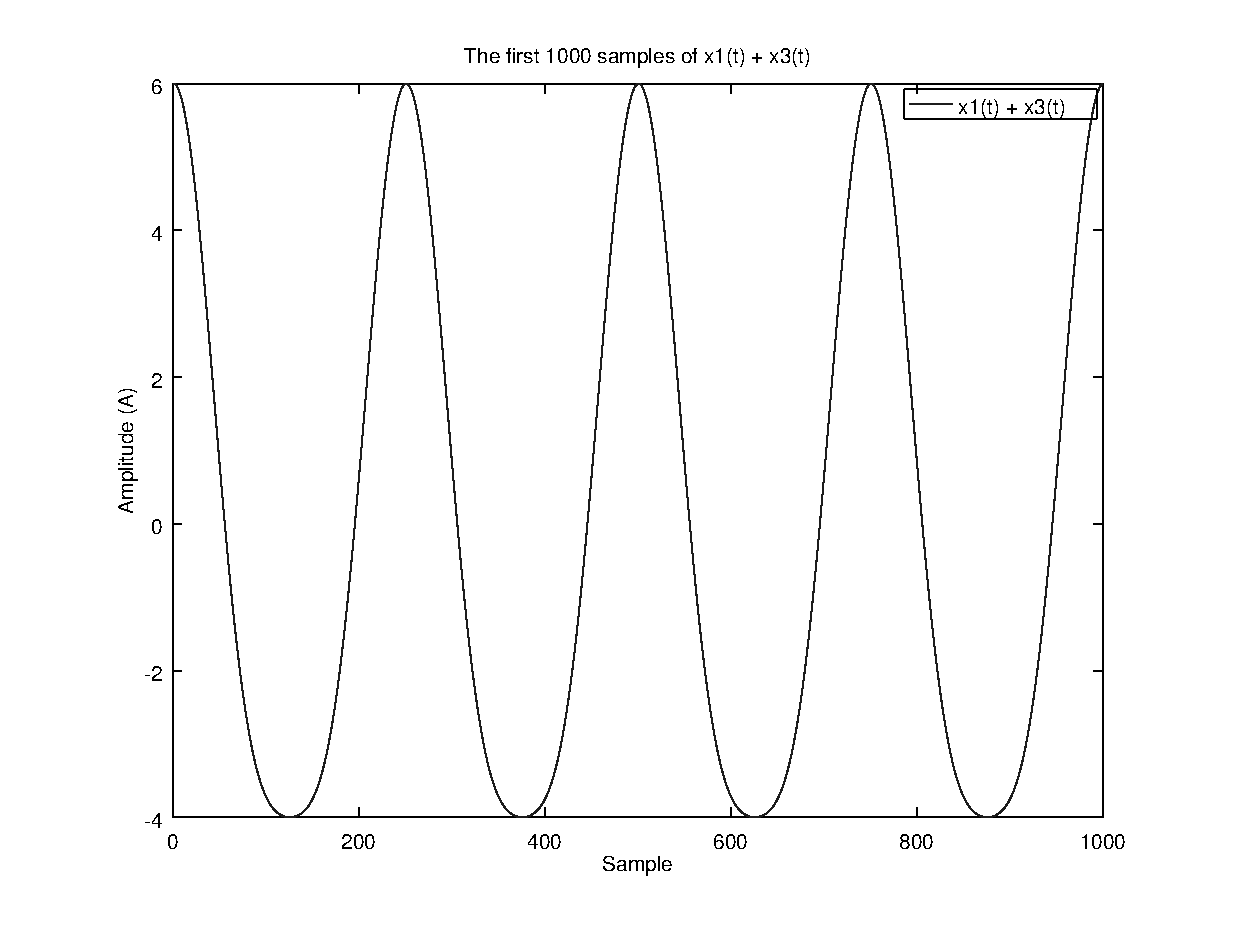
\includegraphics[width=0.7\columnwidth]{plot1E1.eps}\\
  \caption{$z1(t) = x1(t) + x3(t)$}
  \label{fig1e1}
\end{figure}

\begin{figure}[H]
  \centering
  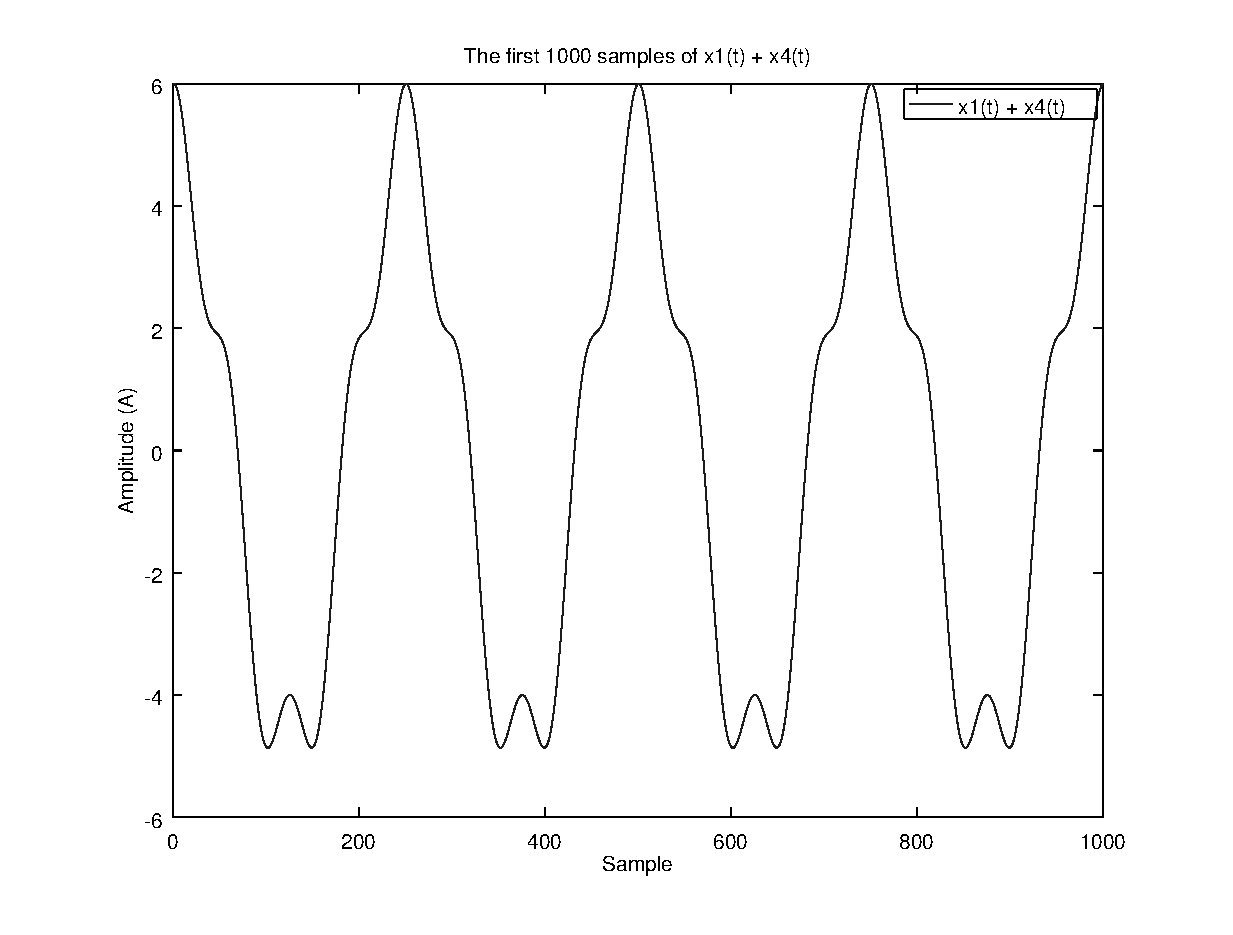
\includegraphics[width=0.7\columnwidth]{plot1E2.eps}\\
  \caption{$z2(t) = x1(t) + x4(t)$}
  \label{fig1e2}
\end{figure}

\begin{figure}[H]
  \centering
  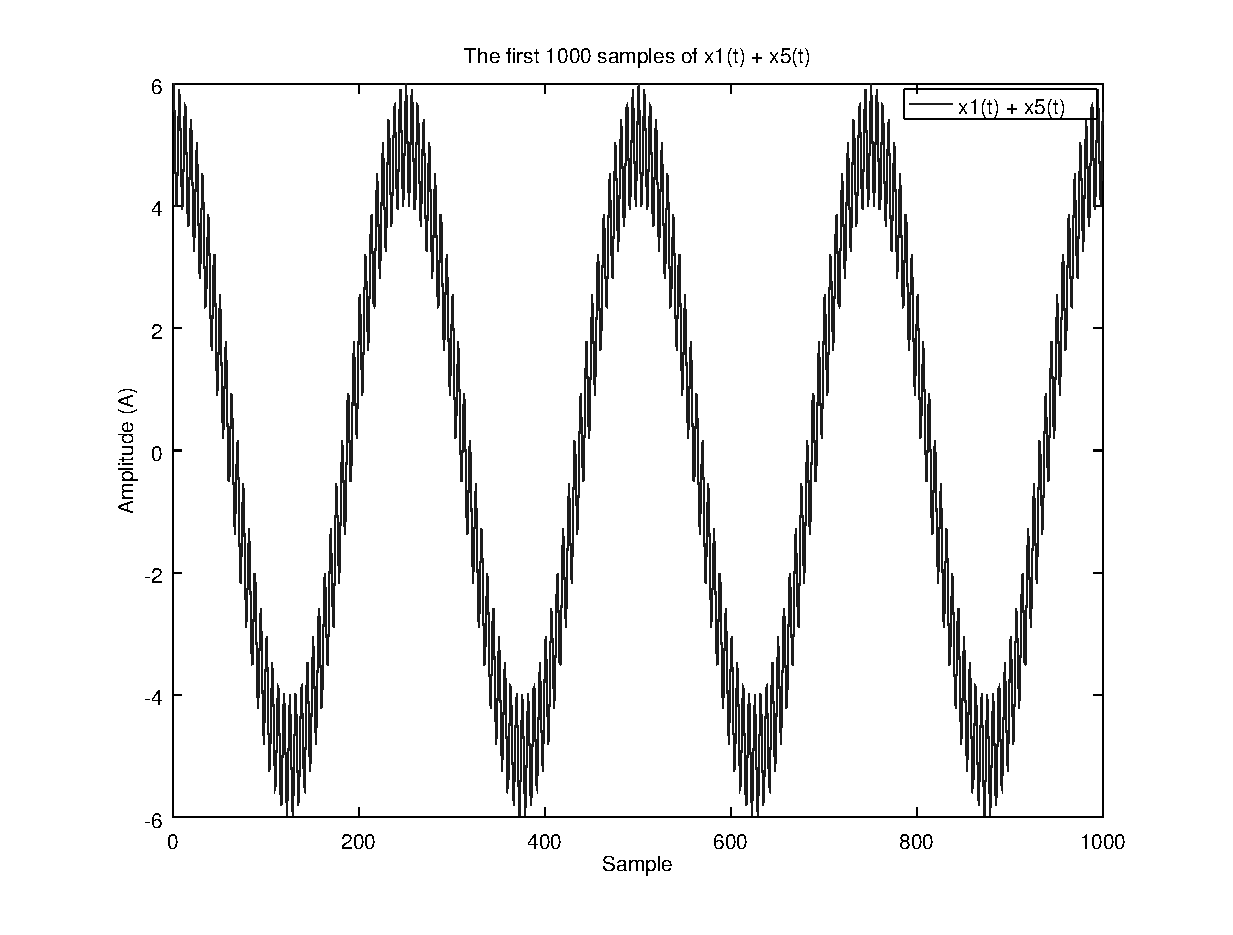
\includegraphics[width=0.7\columnwidth]{plot1E3.eps}\\
  \caption{$z3(t) = x1(t) + x5(t)$}
  \label{fig1e3}
\end{figure}

\newpage
\section*{Appendix}
\appendix
\section{Summing Sinosoids}
\subsection{gensinusoid}
\lstinputlisting{../code/gensinusoid.m}
\subsection{sumsinusoid}
\lstinputlisting{../code/sumsinusoid.m}
\subsection{Verification script 1d}
\lstinputlisting{../code/1d.m}

\section{}

\end{document}
